\documentclass[../main.tex]{subfiles}
\graphicspath{{../images/}}

\begin{document}
\subsection*{Lecture 24: \hfill  3/25/24}
\hrule \vspace{10px}
\section{Solid Body Rotation}

Last Week: Non-inertial Frames
\begin{enumerate}
    \item Just linear acceleration $\vb A$, N2L 
    \begin{align*}
        m \ddot{\vb r} = \vb F - m \vb A
    \end{align*}
    \item Rotating frame: 
    \begin{align*}
        m\ddot{\vb r} = \vb F + 2m\dot{\vb r} \times \Omega + m(\Omega \times \vb r) \times \Omega
    \end{align*}
\end{enumerate}

\subsection*{Solid body} $N$ particles on a continuous distribution
\begin{align*}
    m_\alpha, \qquad \alpha = 1, 2, \dots, N \\
    \vb r_\alpha, \qquad \vb r_\alpha - \vb r_\beta = \text{constant}
\end{align*}
With a center of mass (COM/CM)
\begin{align*}
    \vb R = \frac{1}{M} \sum_\alpha m_\alpha \vb r_\alpha, \qquad M = \sum_\alpha m_\alpha \\
    \vb P = \sum_\alpha m_\alpha \vb v_\alpha = \sum_\alpha m\alpha \dot{\vb r}_\alpha = M \dot{\vb R} \\
    \dot{\vb P} = M \ddot{\vb R} = \vb F_{\text{ext}} 
\end{align*}
\paragraph*{Angular Momentum}
\begin{align*}
    \vb \ell_\alpha &= \vb r_\alpha \times \vb p_\alpha \\
    &= \vb r_\alpha \times m_\alpha \dot{\vb r}_\alpha
\end{align*}
and the total angular momentum
\begin{align*}
    \vb L = \sum_\alpha \vb \ell_\alpha = \sum_\alpha \vb r_\alpha \times m_\alpha \dot{\vb r}_\alpha
\end{align*}
Defining a position $\vb r_\alpha'$ relative to the CM
\begin{align*}
    \vb r_\alpha' = \vb r_\alpha - \vb R, \quad \vb r_\alpha = \vb R + \vb r_\alpha'
\end{align*}
we can rewrite the total angular momentum as
\begin{align*}
    \vb L &= \sum_\alpha m_\alpha(\vb R + \vb r_\alpha') \times (\dot{\vb R} + \dot{\vb r}_\alpha') \\
    &= \sum_\alpha m_\alpha \vb R \times \dot{\vb R} + \sum_\alpha m_\alpha \vb r_\alpha' \times \dot{\vb R} 
    + \sum_\alpha m_\alpha \vb R \times \dot{\vb r}_\alpha' + \sum_\alpha m_\alpha \vb r_\alpha' \times \dot{\vb r}_\alpha' \\
\end{align*}
but since we know that
\begin{align*}
    \vb R &= \frac{1}{M} \sum_\alpha m_\alpha (\vb R + \vb r_\alpha') \\
    &= \frac{1}{M} \sum_\alpha m_\alpha \vb R + \frac{1}{M} \sum_\alpha m_\alpha \vb r_\alpha' \\
    \implies &\sum_\alpha m_\alpha \vb r_\alpha' = 0 \\
    &\sum_\alpha m_\alpha \dot{\vb r}_\alpha' = 0
\end{align*}
so the middle terms of the total angular momentum are zero:
\begin{align*}
    \vb L = M \vb R \times \dot{\vb R} + \sum_\alpha m_\alpha \vb r_\alpha' \times \dot{\vb r}_\alpha'
\end{align*}
which can be re-expressed as
\begin{align*}
    \vb L &= \vb L_{\text{cm}} + \vb L_{\text{rel}} \\
    \vb L_{\text{cm}} &= M \vb R \times \dot{\vb R} \\
    \vb L_{\text{rel}} &= \sum_\alpha m_\alpha \vb r_\alpha' \times \dot{\vb r}_\alpha'
\end{align*}
For example we can consider the earth as a rigid body with angular momentum
\begin{align*}
    \vb L_E = \vb L_{\text{spin}} + \vb L_{\text{orb}}
\end{align*}
\paragraph*{Time derivative of angular momentum} we have two parts
\begin{align*}
    \dot{\vb L}_{\text{cm}} &= M \dot{\vb R} \times \dot{\vb R} + M \vb R \times \ddot{\vb R} \\
    &= M \vb R \times \ext = \vb \Gamma_{\text{cm}} 
\end{align*}
and
\begin{align*}
    \dot{\vb L}_{\text{rel}} &= \sum_\alpha m_\alpha \vb r_\alpha' \times \ddot{\vb r}_\alpha', 
    \quad \ddot{\vb r}_\alpha' = \ddot{\vb r}_\alpha - \ddot{\vb R} \\
    &= \vb \Gamma_{\text{rel}}
\end{align*}
\paragraph*{Energy} The kinetic energy of the system is
\begin{align*}
    T &= \frac{1}{2} \sum_\alpha m_\alpha \dot{\vb r}_\alpha^2 = \frac{1}{2} \sum_\alpha m_\alpha(\dot{\vb R} + \dot{\vb r}_\alpha')^2 \\
    &= \frac{1}{2} \sum_\alpha m_\alpha (\dot{\vb R}^2 + 2\dot{\vb R} \dot{\vb r}_\alpha' + \dot{\vb r}_\alpha'^2) \\
    &= \frac{1}{2} M \dot{\vb R}^2 + \frac{1}{2} \sum_\alpha m_\alpha \dot{\vb r}_\alpha'^2
\end{align*}
and the potential energy is
\begin{align*}
    U = U_{\text{ext}} + U_{\text{int}} = U_{\text{ext}}
\end{align*}
where there is no relative motion between the particles, the internal potential energy is a constant
which can be ignored. 
\paragraph*{Example: Rotating disk} We consider a disk rotating about the $z$-axis with angular velocity
\begin{align*}
    \vb \omega = (0, 0, \omega)
\end{align*}
with a particle with position and velocity
\begin{align*}
    \vb r_\alpha = (x_\alpha, y_\alpha, z_\alpha) \\
    \dot{\vb r}_\alpha = (\dot{x}_\alpha, \dot{y}_\alpha, \dot{z}_\alpha)
\end{align*}
the time derivative of the position vector is
\begin{align*}
    \dot{\vb r}_\alpha = \vb \omega \times \vb r_\alpha = (-\omega y_\alpha, \omega x_\alpha, 0)
\end{align*}
and the angular momentum is
\begin{align*}
    \vb \ell_\alpha &= m_\alpha \vb r_\alpha \times \dot{\vb r}_\alpha = m_\alpha \vb r_\alpha \times (\vb \omega \times \vb r_\alpha) \\
    &= m_\alpha(-\omega x_\alpha z_\alpha, -\omega y_\alpha z_\alpha, \omega (x_\alpha^2 + y_\alpha^2))
\end{align*}
thus the $z$ component of total angular momentum is
\begin{align*}
    L_z = \sum_\alpha m_\alpha \ell_{\alpha, z} = \sum_\alpha m_\alpha \omega(x_\alpha^2 + y_\alpha^2)
    = \omega \sum_\alpha m_\alpha \rho_\alpha^2 = \omega I_z
\end{align*}
where $\rho$ is radius in cylindrical coordinates and $I_z$ is the moment of inertia about the $z$-axis (parallel axis theorem).
The other two components of angular momentum are
\begin{align*}
    L_x = -\sum_\alpha m_\alpha \omega x_\alpha z_\alpha \\
    L_y = -\sum_\alpha m_\alpha \omega y_\alpha z_\alpha
\end{align*}
and since $L_x$ and $L_y$ can be nonzero, that means that $\vb L$ can be in any direction! If we define
the products of inertia 
\begin{align*}
    I_{xz} = -\sum_\alpha m_\alpha x_\alpha z_\alpha \\
    I_{yz} = -\sum_\alpha m_\alpha y_\alpha z_\alpha \\
    I_{zz} = \sum_\alpha m_\alpha (x_\alpha + y_\alpha)^2
\end{align*}
we define the total angular momentum as
\begin{align*}
    \vb L &= I \cdot \vb \omega \\
    &= (I_{xz} \cdot \omega_z, I_{yz} \cdot \omega_z, I_{zz} \cdot \omega_z)
\end{align*}

\newpage
\subsection*{Lecture 25: \hfill 3/27/24}
\hrule \vspace{10px}

\paragraph*{HW 8 Hint} For a puck on a rotating table
\begin{align*}
    \ddot{\vb r} &= 2\dot{\vb r} \times \vb \Omega + (\vb \Omega \times \vb r) \times \vb \Omega
\end{align*}
where the first term points inward, and the second term points outward. Since
\begin{align*}
    \dot{\vb r} = - \vb \Omega \times \vb r \\
    \implies \ddot{\vb r} = - r \Omega^2
\end{align*}
or the centripetal acceleration. 

\subsection*{Inertia Tensor}
For a general rigid body, we define the angular velocity
\begin{align*}
    \vb \omega = (\omega_x, \omega_y, \omega_z) 
\end{align*}
the angular momentum
\begin{align*}
    \vb L = \sum_\alpha \vb \ell_\alpha = \sum_\alpha \vb r_\alpha \times m_\alpha \dot{\vb r}_\alpha 
        = \sum_\alpha m_\alpha \vb r_\alpha \times \dot{\vb r}_\alpha 
\end{align*}
where $\dot{\vb r}_\alpha = \vb \omega \times \vb r_\alpha$. Using the BAC-CAB rule we can write
\begin{align*}
    \vb r \times (\vb \omega \times \vb r) = \vb \omega(\vb r \cdot \vb r) - \vb r(\vb r \cdot \vb \omega)
\end{align*}
so
\begin{align*}
    L_x &= \sum_\alpha m_\alpha(\omega_x (x_\alpha^2 + y_\alpha^2+ z_\alpha^2) 
    - x(\cancel{\omega_x} x_\alpha + \omega_y y_\alpha + \omega_z z_\alpha)) \\
    &= \sum_\alpha m_\alpha(\omega_x(y^2 + z^2)) - m_\alpha x_\alpha y_\alpha \omega_y 
        - m_\alpha x_\alpha z_\alpha \omega_z
\end{align*}
where we define the products of inertia for $\vb L = I \vb \omega$:
\begin{align*}
    L_i &= \sum_j^3 I_{ij} \omega_j \\
    L_x = I_{xx} \omega_x + I_{xy} \omega_y + I_{xz} \omega_z
\end{align*}
where
\begin{align*}
    I_{xx} = \sum_\alpha m_\alpha(y_\alpha^2 + z_\alpha^2) \\
    I_{xy} = -\sum_\alpha m_\alpha x_\alpha y_\alpha = I_{yx} \\
    I_{xz} = -\sum_\alpha m_\alpha x_\alpha z_\alpha = I_{zx}
\end{align*}
for the the first row, and
\begin{align*}
    I_{yy} = \sum_\alpha m_\alpha(x_\alpha^2 + z_\alpha^2) \\
    I_{yx} = -\sum_\alpha m_\alpha y_\alpha x_\alpha \\
    I_{yz} = -\sum_\alpha m_\alpha y_\alpha z_\alpha = I_{zy}
\end{align*}
similarly for the second row and third row. These creates a real $3 \times 3$ matrix that is 
symmetric or
\begin{align*}
    I = I^T
\end{align*}
\paragraph*{Example: Dumbell in the $yz$ plane} The masses are placed at $(0, \pm y_0, z)$, so the 
products of inertia are
\begin{align*}
    I_{zz} = 2m y_0^2, \quad I_{xx} = 2m(y_0^2 + z_0^2), \quad I_{yy} = 2m z_0^2
\end{align*}
and for the nondiagonal terms
\begin{align*}
    I_{xy} = 0 = I_{xz},\quad I_{yz} = 0 \dots
\end{align*}
are all zero. Thus we create the inertia tensor
\begin{align*}
    I = \begin{pmatrix}
        I_{xx} & I_{xy} & I_{xz} \\
        I_{yx} & I_{yy} & I_{yz} \\
        I_{zx} & I_{zy} & I_{zz}
    \end{pmatrix}
\end{align*}
\paragraph*{Another example: A disk on the $xy$ plane} The disk has radius $R$ and mass $M$ lying
on the $xy$ plane at $z = z_0$. The mass is distributed evenly, so
\begin{align*}
    m_\alpha &= \dd{m} = \rho R \dd{\theta} \\
    M &= \int \dd{m} = \int_0^{2\pi} \rho R \dd{\theta} = 2\pi \rho R^2 \\
    \implies \rho &= \frac{M}{2\pi R^2}
\end{align*}
The products of inertia are now calcaulable:
\begin{align*}
    I_{zz} &= \sum_\alpha m_\alpha (x_\alpha^2 + y_\alpha^2) = 0 \\
        &= \int_0^{2\pi} \rho R \dd{\theta} (x^2 + y^2) \qquad R = x^2 + y^2 \\
        &= \int_0^{2\pi} \rho R^3 \dd{\theta} = 2\pi \rho R^3 = 2\pi \frac{M}{2\pi R^2} R^3 = MR
\end{align*}
and the other products
\begin{align*}
    I_{xx} &= \sum_\alpha m_\alpha (y_\alpha^2 + z_\alpha^2) \\
        &= \int_0^{2\pi} \rho R \dd{\theta} (y^2 + z_0^2) \\
        &= \int_0^{2\pi} \rho R \dd{\theta} (R^2\cos^2\theta + z_0^2) \\
        &= Mz_0^2 + \int_0^{2\pi} \rho R^3 \cos^2\theta \dd{\theta} \\
        &= Mz_0^2 + \pi \rho R^3 \\
        &= Mz_0^2 + \pi \frac{M}{2\pi R^2} R^3 = Mz_0^2 + \frac{M}{2}R^2
\end{align*}
we can see the familar term for the moment of inertia of a disk $I = \frac{1}{2}MR^2$ which is 
shifted. The cross terms are
\begin{align*}
    I_{yz} = -\sum_\alpha m_\alpha y_\alpha z_0 = 0 = I_{xz} \\
    I_{xy} = 0 \dots
\end{align*}
where can see that the average of $y$ is zero for the first term, and we see that all the cross
terms are zero as well.
\paragraph*{Final Example: A cube with corner at the origin} Given the side length $a$ we know that
the mass is simply
\begin{align*}
    M = \rho a^3,\quad \rho = \frac{M}{a^3}
\end{align*} 
and the products of inertia are
\begin{align*}
    I_{xy} &= -\int_0^a \dd{x} \int_0^a \dd{y} \int_0^a \dd{z} \rho x y \\
    &= -\frac{1}{2} a^2 \cdot \frac{1}{2}a^2 \cdot a \cdot \rho = -\frac{1}{4}Ma^2
\end{align*}
and the other cross terms are the same as well
\begin{align*}
    I_{yz} = I_{xz} = -\frac{1}{4}Ma^2
\end{align*}
The diagonal terms
\begin{align*}
    I_{zz} &= \iiint_0^a \rho (x^2 + y^2) \dd{V} \\
    &= \frac{1}{3} a^3 \cdot a \cdot a \cdot \rho + a \cdot \frac{1}{3} a^3 \cdot a \cdot \rho \\
    &= \frac{2}{3} Ma^2 = I_{xx} = I_{yy} 
\end{align*}
this gives us the inertia tensor
\begin{align*}
    I = Ma^2 \begin{pmatrix}
        \frac{2}{3} & -\frac{1}{4} & -\frac{1}{4} \\[6pt]
        -\frac{1}{4} & \frac{2}{3} & -\frac{1}{4} \\[6pt]
        -\frac{1}{4} & -\frac{1}{4} & \frac{2}{3}
    \end{pmatrix}
\end{align*}
The symmetry of the axes tell us how lopsided or asymmetrical the object is.

\newpage
\subsection*{Lecture 26: \hfill 3/29/24}
\hrule \vspace{10px}

\paragraph*{Inertial Tensor} We can define the inertial product
\begin{align*}
    I_{ij} = \sum_\alpha m_\alpha (r_\alpha^2 \delta_{ij} - r_{\alpha, i} r_{\alpha, j})
\end{align*}
where $\delta_{ij}$ is the kronicker delta. We know that $I$ in $3 \times 3$ is real and symmetric. 
$I$ is diagonalizeable
\begin{align*}
    \exists \qqtext{3 axes} \vu e_1, \vu e_2, \vu e_3 
\end{align*}
such that $I$ is diagonal i.e.
\begin{align*}
    I = \mqty(\lambda_1 & & \\ & \lambda_2 & \\ & & \lambda_3)
\end{align*}
Where
\begin{align*}
    \lambda_1,\quad \lambda_2,\quad \lambda_3
\end{align*}
are the principle moments of inertia and the principle axes are
\begin{align*}
    \vu e_1, \vu e_2, \vu e_3
\end{align*}
Thus the matrix rows are in the form
\begin{align*}
    I \vu e_i = \lambda_i \vu e_i
\end{align*}
And $I$ is diagonalized by rotation. To solve a diagonization problem we have to solve for $\lambda$
by using the angular momentum equation
\begin{align*}
    \vb L = I \vb \omega = \lambda \vb \omega \\
    I \omega - \lambda \omega = 0 \\
    (I - \lambda \mathbb{1}) \vb \omega = 0 \\
    \implies \det(I - \lambda \mathbb{1}) = 0
\end{align*}
which gives us the matrix
\begin{align*}
    \begin{vmatrix}
        I_{xx} - \lambda & I_{xy} & I_{xz} \\
        I_{yx} & I_{yy} - \lambda & I_{yz} \\
        I_{zx} & I_{zy} & I_{zz} - \lambda
    \end{vmatrix} = 0
\end{align*}
so from the cube example we have
\begin{align*}
    I = \frac{Ma^2}{12} \begin{pmatrix}
        8 & -3 & -3 \\
        -3 & 8 & -3 \\
        -3 & -3 & 8
    \end{pmatrix} \qquad \mu = \frac{Ma^2}{12}
\end{align*}
thus
\begin{align*}
    \det(I - \lambda \mathbb{1}) = \begin{vmatrix}
        8\mu - \lambda & -3\mu & -3\mu \\
        -3\mu & 8\mu - \lambda & -3\mu \\
        -3\mu & -3\mu & 8\mu - \lambda
    \end{vmatrix}
\end{align*}
To solve this, we can use some tricks:
\begin{itemize}
    \item Circular matrix: Since the sum of every row is the same
    \begin{align*}
        \sum_j I_{ij} = \text{constant} = \lambda_1
    \end{align*}
    \item Trace of a matrix (sum of diagonal entries) 
    \begin{align*}
        \Tr(I) &= I_{xx} + I_{yy} + I_{zz} \\
            &= \sum_i \lambda_i
    \end{align*}
    \item Determinant of a matrix
    \begin{align*}
        \det(I) &= \lambda_1 \lambda_2 \lambda_3
    \end{align*}
\end{itemize}
so
\begin{align*}
    \lambda_1 = 2 \mu,\quad \Tr(I) = 24\mu,\quad \det(I) = 242\mu^3
\end{align*}
so form the other two equations
\begin{align*}
    \lambda_1 + \lambda_2 + \lambda_3 = 24\mu \\
    \lambda_2 \lambda_3 = 22\mu^2
\end{align*}
and
\begin{align*}
    \lambda_1 \lambda_2 \lambda_3 = 242\mu^3 \\
    \lambda_2 \lambda_3 = 121\mu^2
\end{align*}
which gives us
\begin{align*}
    \lambda_2 = \lambda_3 = 11\mu
\end{align*}
And to get the principle axes we can use the eigenvectors of the matrix
\begin{align*}
    \lambda \vu e_1 = I \vu e_1 \\
    \mqty(8\mu & -3\mu & -3\mu \\ -3\mu & 8\mu & -3\mu \\ -3\mu & -3\mu & 8\mu) 
    \mqty(w_1 \\ w_2 \\ w_3) = 2\mu \mqty(w_1 \\ w_2 \\ w_3) \\
    \mqty(6\mu & -3\mu & -3\mu \\ -3\mu & 6\mu & -3\mu \\ -3\mu & -3\mu & 6\mu)
    \mqty(w_1 \\ w_2 \\ w_3) = 0
\end{align*}
and we can guess a solution from the first two rows
\begin{align*}
    6\mu w_1 - 3\mu w_2 - 3\mu w_3 = 0 \\
    6\mu w_2 - 3\mu w_1 - 3\mu w_3 = 0
\end{align*}
summing these two equations gives us
\begin{align*}
    9\mu w_1 - 9\mu w_2 = 0 \implies w_1 = w_2 = w_3
\end{align*}
and we can normalize the vector to get
\begin{align*}
    \vu e_1 = \frac{1}{\sqrt{3}} \mqty(1 \\ 1 \\ 1)
\end{align*}
for the second unit vector
\begin{align*}
    I \vu e^2 = \lambda_2 \vu e^2 \\
    \mqty(-3\mu & -3\mu & -3\mu \\ -3\mu & -3\mu & -3\mu \\ -3\mu & -3\mu & -3\mu)
    \mqty(w_1 \\ w_2 \\ w_3) = 0
\end{align*}
where we can guess that
\begin{align*}
    \frac{1}{\sqrt{3}} (w_1 + w_2 + w_3) = 0 \leftrightarrow \vb \omega \cdot \vu e_1 = 0
\end{align*}
We call the new basis vectors of the principle axes the \emph{Body Frame}: $\vu e_1, \vu e_2, \vu e_3$.
The \emph{Space Frame} is the original frame of reference: $\vu x, \vu y, \vu z$. And in the body 
frame
\begin{align*}
    \vb L_{\text{body}} = (\lambda_1 \omega_1, \lambda_2 \omega_2, \lambda_3 \omega_3)
\end{align*}
Note that this may point in a different direction than the angular velocity vector.

\newpage
\subsection*{Lecture 27: \hfill 4/1/24}
\hrule \vspace{10px}
If $\vb \omega = \omega e_3$
\begin{align*}
    \vb L = I \vb \omega = \lambda_3 \omega_3 \vu e_1
\end{align*}
\begin{figure}[ht]
    \centering
    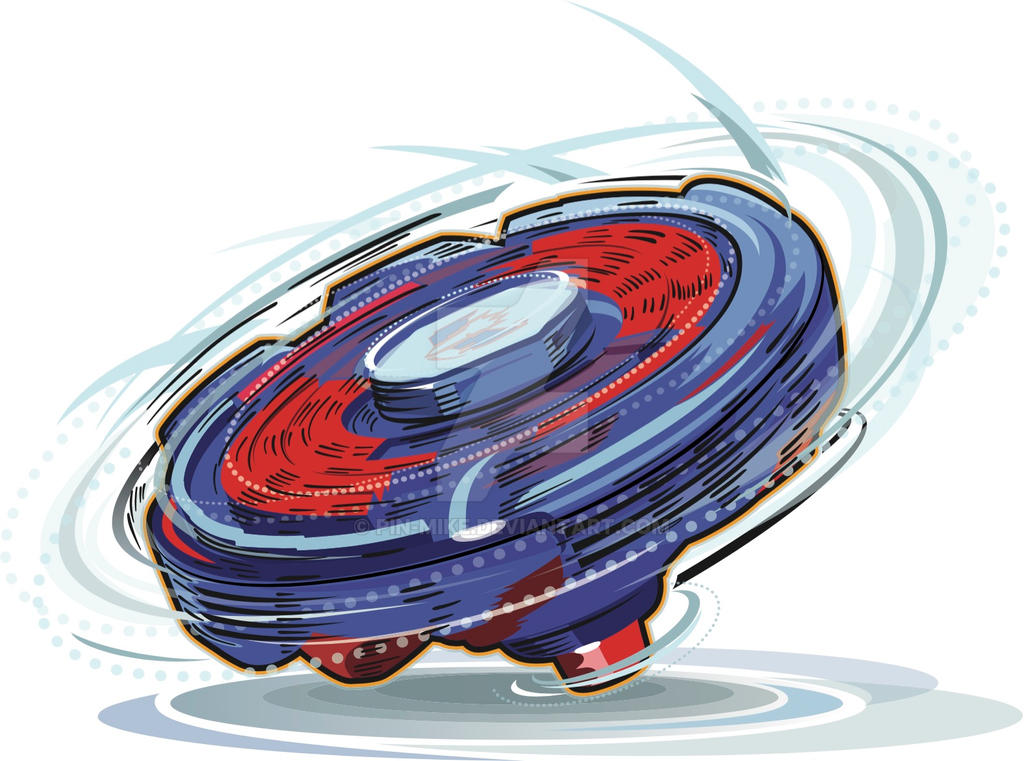
\includegraphics[width=0.5\linewidth]{beyblade.jpeg}
    \caption{The body frame has $\vu e_3$ point in the direction of the spinning beyblade.}
\end{figure}

Since $\dot{\vb L} = \vb \Gamma = \vb R \times M \vb g$ where a nonzero torque allows the body to 
precess. If we look at the torque more carefully given
\begin{align*}
    \vb R = R \vu  e_1, \quad \vb g = -g \vu z
\end{align*}
\begin{align*}
    \lambda_3 \omega_3 \dot{\vu e}_1 &= MgR \vu z \times \vu e_3 \\
    \dot{\vu e}_3 &= \frac{MgR}{\lambda_3 \omega_3} \vu z \times \vu e_3 = \Omega \times \vu e_3
\end{align*}
\paragraph*{Euler's Equations} 
\begin{itemize}
    \item Body Frame $\vu e_1, \vu e_2, \vu e_3 \qquad S$ 
    \item Space Frame $\vu x, \vu y, \vu z \qquad S_0$
\end{itemize}
\begin{align*}
    \qt(\dv{\vb L}{t})_{\text{space}} &= \qt(\dv{\vb L}{t})_{\text{body}} + \vb \omega \times \vb L \\
    &= \dot{\vb L} + \omega \times \vb L = \vb \Gamma
\end{align*}
where
\begin{align*}
    \vb L &= \lambda_1 \omega_1 \vu e_1 + \lambda_2 \omega_2 \vu e_2 + \lambda_3 \omega_3 \vu e_3 \\
    \vb \omega &= \omega_1 \vu e_1 + \omega_2 \vu e_2 + \omega_3 \vu e_3
\end{align*}
Keep in mind that the dot product is not always zero(only if $\vb L = \lambda \vb \omega$ i.e. a
sphere).
\begin{align*}
    \vb \omega \times \vb L &= 
    \mqty(\vu e_1 & \vu e_2 & \vu e_3 \\
         \omega_1 & \omega_2 & \omega_3 \\ 
        \lambda_1 \omega_1 & \lambda_2 \omega_2 & \lambda_3 \omega_3) \\
    &= \vu e_1 [\omega_2 \omega_3 (\lambda_3 - \lambda_2)] \\
    &+ \vu e_2 [\omega_3 \omega_1 (\lambda_1 - \lambda_3)] \\
    &+ \vu e_3 [\omega_1 \omega_2 (\lambda_2 - \lambda_1)]
\end{align*}
so the three components of the torque(or Euler's equations) are 
\begin{align*}
    \Gamma_1 &= \lambda \dot{\omega}_1 + (\lambda_3 - \lambda_2) \omega_2 \omega_3 \\
    \Gamma_2 &= \lambda \dot{\omega}_2 + (\lambda_1 - \lambda_3) \omega_3 \omega_1 \\
    \Gamma_3 &= \lambda \dot{\omega}_3 + (\lambda_2 - \lambda_1) \omega_1 \omega_2
\end{align*}
\paragraph*{Zero Torque Case} Setting the RHS to zero and moving the lambda terms
\begin{align*}
    \lambda_1 \dot \omega_1 &= (\lambda_2 - \lambda_3) \omega_2 \omega_3 \\
    \lambda_2 \dot \omega_2 &= (\lambda_3 - \lambda_1) \omega_3 \omega_1 \\
    \lambda_3 \dot \omega_3 &= (\lambda_1 - \lambda_2) \omega_1 \omega_2
\end{align*}
Example: Let $\vb \omega = \omega_3 \vu e_3, \quad \vb L = \lambda_3 \vb \omega = \lambda_3 \omega_3 \vu e_3$
thus
\begin{align*}
    \omega_1 = \omega_2 = 0
\end{align*}
and the RHS for all three equations are zero. Thus the body keeps rotating in the same direction. 

If initially $\vb \omega = \sum_i^3 \omega_i \vu e_i$ we have a lot of motion in any direction.
\paragraph*{Small Deviation} $\vb L = \lambda_3 \omega_3 \vu e_3$ add small $\omega_1, \omega_2$: 
The third equation would be approximately zero, i.e., $\lambda_3 \dot \omega_3 = 0$ is constant. 
We are then left with two equations
\begin{align*}
    \lambda_1 \dot \omega_1 &= (\lambda_2 - \lambda_3) \omega_2 \omega_3 \\
    \lambda_2 \dot \omega_2 &= (\lambda_3 - \lambda_1) \omega_3 \omega_1
\end{align*}
where we have cross terms in the coupled equations. Taking the time derivative of the first equation
\begin{align*}
    \ddot \omega_1 &= -\qt[\frac{(\lambda_3 - \lambda_2)(\lambda_3 - \lambda_1) \omega_3^2}{\lambda_2 \lambda_1}] \omega_1 \\
    \ddot x &= - \frac{k}{m} x = - \omega_0^2 x
\end{align*}
where this resembles a harmonic oscillator so
\begin{align*}
    \omega_0^2 = \frac{(\lambda_3 - \lambda_2)(\lambda_3 - \lambda_1)}{\lambda_2 \lambda_1} \omega_3^2
\end{align*}
but the caveat is that the term must be positive or
\begin{align*}
    \lambda_3 > \lambda_2, \lambda_1
\end{align*}
or both negative
\begin{align*}
    \lambda_3 < \lambda_2, \lambda_1
\end{align*}
for $\omega_0^2 > 0$ 
if
\begin{align*}
    \lambda_1 < \lambda_3 < \lambda_2 \qquad \omega_0^2 < 0
\end{align*}

\newpage 
\begin{figure}[ht]
    \centering
    \includegraphics[width=0.8\linewidth]{book.png}
    \caption{Book and its three principal moments of inertia.}
\end{figure}

Looking at a book, we can see that from the 3 principal moments of inertia, rotating around the 
largest moment (pointing out of the page) is stable, and rotating around the two smaller moments are
unstable. 

\newpage
\subsection*{Lecture 28: \hfill 4/3/24}
\hrule \vspace{10px}
For a book.
\begin{align*}
    \lambda_1 \neq \lambda_2 \neq \lambda_3 \qqtext{initially} \vb \omega = \omega_3 \vu e_3
\end{align*}
Adding a small $\omega_1, \omega_2$ where
\begin{align*}
    \ddot \omega_1 &= -\qt[\frac{(\lambda_3 - \lambda_1)(\lambda_3 - \lambda_2)}{\lambda_1 \lambda_2}\omega_3^2] \omega_1
\end{align*}
We can see in the largest moment of inertia, a rotation is stable, but rotation in $\lambda_1$ in the figure
leads to an unstable rotation, i.e., the book when tossed will rotate around the other axes.
\paragraph*{Symmetric top} $\lambda_1 = \lambda_2 \neq \lambda_3$
Then from the Euler's equations
\begin{align*}
    \lambda_3 \dot \omega_3 &= 0
\end{align*}
and using $\lambda_1 = \lambda_2$ the other two equations are
\begin{align*}
    \lambda_1 \dot \omega_1 &= (\lambda_1 - \lambda_3) \omega_3 \omega_2 \\
    \lambda_1 \dot \omega_2 &= -(\lambda_1 - \lambda_3) \omega_3 \omega_1
\end{align*}
and using
\begin{align*}
    \Omega_b = \frac{\lambda_1 - \lambda_3}{\lambda_1} \omega_3
\end{align*}
the equations are
\begin{align*}
    \dot \omega_1 &= \Omega_b \omega_2 \\
    \dot \omega_2 &= -\Omega_b \omega_1
\end{align*}
Which can be solved using the solution 
\begin{align*}
    \eta &= \omega_1 + i \omega_2 \\
    \dot \omega_1 + i \dot \omega_2 &= \Omega_b \omega_2 - i \Omega_b \omega_1 \\
    &= \Omega_b (\omega_2 -i\omega_1) \\
    &= i\Omega_b (i\omega_2 - \omega_1) \\
    \dot \eta &= - \Omega_b \eta \implies \eta = \eta_0 e^{-i\Omega_b t}
\end{align*}
so
\begin{align*}
    \omega_1 &= \omega_0 \cos(\Omega_b t) \\
    \omega_2 &= \omega_0 \sin(\Omega_b t)
\end{align*}
where $\Omega_b$ is the free precession frequency (zero torque still results in precession). 

\newpage
\subsection*{Euler Angles} Goal: To find the Lagrangian for a rotating body.
We can describe the orientation of the body axes (principal moments) within a space frame:
The three angles $\phi, \theta, \psi$ 

\begin{figure}[ht]
    \centering
    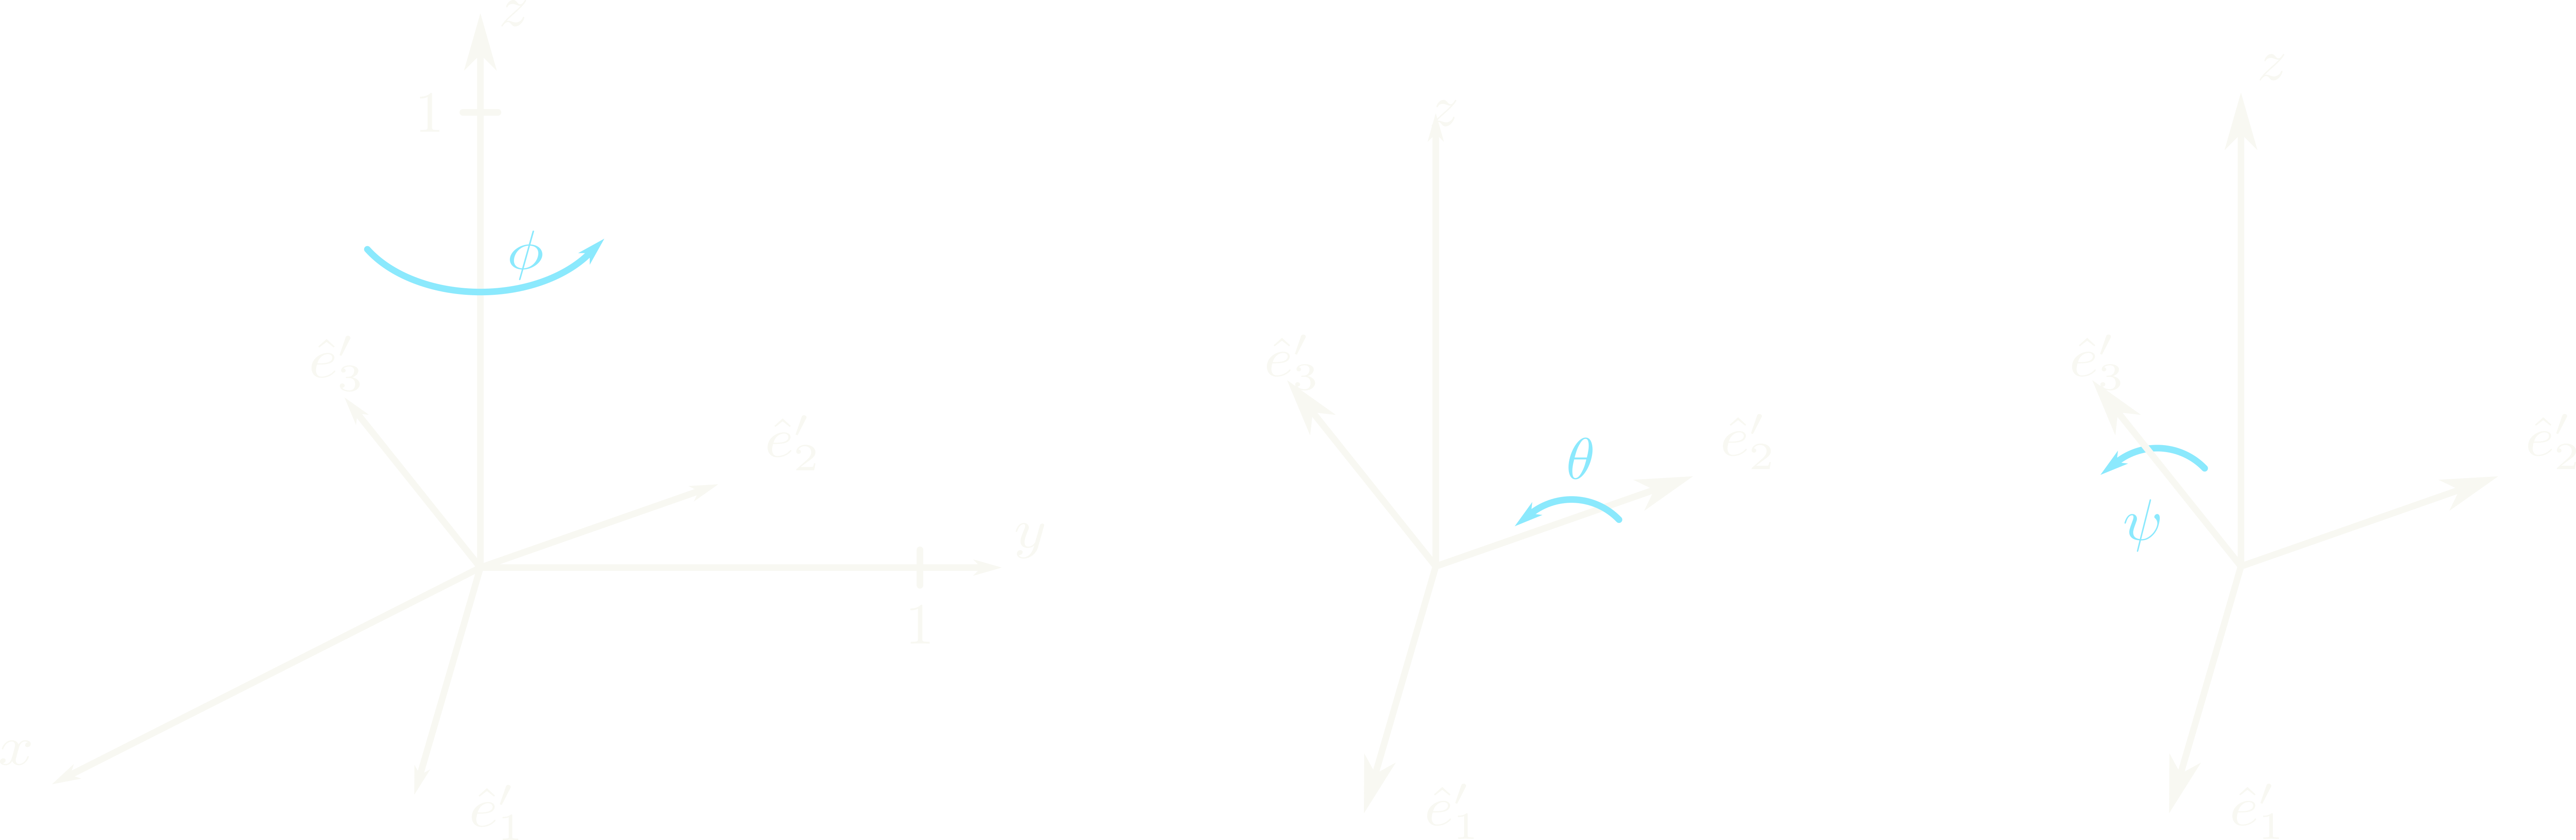
\includegraphics[width=0.8\linewidth]{eulerangle.png}
    \caption{Euler angles $\phi, \theta, \psi$. We can relate $\cos\theta = \vu e_3 \cdot \vu z$}
\end{figure}

First you rotate around $\vu z$ by $\psi$, then around $\vu e_2'$ by $\theta$, and finally 
around $\vu e_3'$ by $\phi$.

The three operations can be defined as the angular velocity vector sum
\begin{align*}
    \vb \omega &= \vb \omega_a + \omega_b + \omega_c \\
    \vb \omega_a &= \dot \phi \vu z \\
    \vb \omega_b &= \dot \theta \vu e_2' \\
    \vb \omega_c &= \dot \psi \vu e_3' \\
    \vb \omega &= \dot \phi \vu z + \dot \theta \vu e_2' + \dot \psi \vu e_3'
\end{align*}
For the symmetric top we can discount the third step, and if $\lambda_1 = \lambda_2$ then
\begin{align*}
    \vu e_1 &= \vu e_1' \\
    \vu e_2 &= \vu e_2'
\end{align*}
so
\begin{align*}
    \vu z &= \vu e_3 \cos \theta - \vu e_1' \sin\theta
\end{align*}
which gives the angular velocity vector
\begin{align*}
    \vb \omega &= -\dot\phi \sin\theta \vu e_1' + \dot\theta \vu e_1' + (\dot \psi + \dot \phi \cos\theta) \vu e_3' \\
    &=\omega_1 \vu e_1' + \omega_2 \vu e_2' + \omega_3 \vu e_3'
\end{align*}
The angular momentum vector is then 
\begin{align*}
    \vb L &= I \vb omega \\
    &= \lambda_1 \omega_1 + \lambda_2 \omega_2 + \lambda_3 \omega_3
\end{align*}
and the Kinetic energy is 
\begin{align*}
    T &= \frac{1}{2} \omega \cdot \vb L \\
    &= \frac{1}{2} [\lambda_1 (\dot \phi^2 \sin^2\theta + \dot\theta^2) + \lambda_3 (\dot\psi + \do\phi \cos\theta)^2]
\end{align*}
To find the potential energy we use the CM $R$ and gravity $\vb g = - g \vu z$:
\begin{align*}
    U = Mgh = MgR \cos\theta
\end{align*}
where we can find the Lagrangian $\lagr = T - U$

\newpage
\subsection*{Lecture 29: \hfill 4/5/24}
\hrule \vspace{10px}

\paragraph*{Euler Angles cont'd} For a rotating rigid body where $\lambda_1 = \lambda_2$:
\begin{align*}
    \lagr &= T - U \\  
    &= \frac{1}{2} \lambda_1 (\dot \phi^2 \sin^2\theta + \dot\theta^2) 
    + \frac{1}{2} \lambda_3 (\dot\psi + \do\phi \cos\theta)^2
    - MgR \cos\theta
\end{align*}
And the two conserved quantities are $\psi$ and $\phi$: Since $\lagr$ is independent of $\psi,\phi$
\begin{align*}
    p_\phi = \pdv{\lagr}{\dot \phi} &= \lambda_1 \dot \phi \sin^2\theta + \lambda_3 (\dot\psi + \dot\phi \cos\theta) \cos\theta = \text{constant} = L_z \\
    p_\psi = \pdv{\lagr}{\dot \psi} &= \lambda_3 (\dot\psi + \dot\phi \cos\theta) = \text{constant} = L_3
\end{align*}
So the momentum is conserved in the $z$ direction and the $3$ direction. Two get the third equation
we can use the Euler-Lagrange equations for $\theta$:
\begin{align*}
    \pdv{\lagr}{\theta} &= \dv{t}(\pdv{\lagr}{\dot\theta}) \\
    \lambda_1 \ddot{\theta} &= \lambda_1 \dot \phi^2 \sin\theta \cos\theta 
        - \lambda_3 (\dot \psi + \dot\phi \cos\theta) \dot\phi \sin\theta + MgR \sin\theta
\end{align*}
or
\begin{align*}
    \frac{L_z - L_3 \cos\theta}{\lambda_1 \sin^2\theta} = \dot \theta
\end{align*}
Assuming that $\theta = \text{constant}, \quad \dot\phi = \Omega$. We can also see that 
$(\dot\psi + \dot\phi \cos\theta) = \omega_3$, so
\begin{align*}
    0 &= \lambda_1 \Omega^2 \sin\theta \cos\theta - \lambda_3 \omega_3 \Omega \sin\theta + MgR \sin\theta \\
    &= \lambda_1 \Omega^2 \cos\theta - \lambda_3 \omega_3 \Omega + MgR
\end{align*}
and since everything except $\Omega$ is constant we can solve using the quadratic formula:
\begin{align*}
    \Omega &= \frac{\lambda_3 \omega_3 \pm \sqrt{(\lambda_3 \omega_3)^2 - 4\lambda_1 MgR \cos\theta}}{2\lambda_1 \cos\theta}
\end{align*}
and for $\omega_3 \gg 1$ we can find the free precession frequency $\Omega_1$:
\begin{align*}
    \Omega_1 = \frac{\lambda_3 \omega_3}{\lambda_1 \cos\theta} \\
    \Omega_2 = \frac{MgR}{\lambda_3 \omega_3} 
\end{align*}
where $\Omega_2$ is the precession due to gravity. Looking at the Lagrangian but rewriting as
\begin{align*}
    \lagr &= \frac{1}{2} \lambda_1 \dot\theta^2 + \frac{(L_z - L_3 \cos\theta)^2}{2\lambda_1 \sin^2\theta}
    + \frac{L_3^2}{2\lambda_3} + MgR \cos\theta \\
    &= \frac{1}{2} \lambda_1 \dot\theta^2 + U_{\text{eff}}
\end{align*}
where $U_{\text{eff}}$ is the effective potential energy. Theta ranges from $0 \to \pi$ 
(From the $\sin\theta$ term), and as $\theta \to 0, \pi$ the potential energy goes to infinity!
\end{document}